\chapter{Monte Carlo Simulation}
\label{cap:montecarlo}

% Bayesian probabilities !!!
The modern version of the Monte Carlo method dates back to the application of the first computers during the years 1940-45 with the purpose of computing neutron diffusion in atomic bombs.

The Monte Carlo approach was primarily promoted by physics researchers Stanislaw Ulam, Nicholas Metropolis and John von Neumann. They were well aware of the potential of such technique but it was only with the first electronic computer, the ENIAC, which was able to solve differential equations at a tremendous, and so far inconceivable, speed, that Monte Carlo method was eventually triggered.

The name Monte Carlo refers to a famous casino in Monaco where Ulam's uncle used to indulge his gambling passion. 
The characteristics of randomness and the repetitive nature of many processes correspond with the games played in a casino. Note that the famous roulette wheel is one of the simplest mechanical devices to generate random variables.

Monte Carlo tools find their application mostly in cases where the inherent complexity of a problem makes the use of other techniques impossible or where no analytically tractable solution exists.
They are are widely used in many fields: Engineering, Physics, Computational biology, Computer graphics, Applied statistics and Artificial intelligence for games.

It started to be en vogue in financial mathematics in the 1980s, particularly when the theories of the random walk of asset prices came up.

In this Chapter this very important technique is reviewed and presented beside some applications.

\section{The Algorithm}
\label{whats-monte-carlo-simulation}

Monte Carlo (MC) method is a numerical approach that simulate a process by replacing every source of uncertainty by random numbers sampled from appropriate distributions (PDF). This is a clear improvement with respect to just replacing the uncertain variable with a single average number.

The model is processed many times with different sampling of the random variables and once the simulation is completed, the results are either averaged as an estimate or their distribution is provided.

Note that depending upon the number of uncertainties and their ranges, a Monte Carlo simulation could involve thousands or even millions of recalculations before it is completed.

A MC method/algorithm then can be summarized as follows:

\begin{itemize}
\item  identify all the source of uncertainty of the problem and define their domain $\Omega$ of possible inputs (probability distributions for the inputs);
\item sample random inputs from the domain $\Omega$;
\item compute the model output based on the randomly generated inputs;
\item repeat the experiment $N$ times and aggregate the results.
\end{itemize}

Imagine to simulate the results of rolling a die: the only variable is the die outcome, so $\Omega =1,2,3,4,5,6$ and the outcome probability is a uniform distribution (i.e. we are using a fair die and outcomes are equiprobable). Hence the simulation consists of sampling uniform distributed integers between 1 and 6.

\section{Pseudo-Random Numbers}
\label{pseudo-random-numbers}

The need of generating random inputs during a MC simulation requires large amounts of \emph{random numbers} to be generated, and it was their use that spurred the development of \emph{pseudo-random number generators}. 

Nowadays every programming language has libraries that allow to produce huge series of random numbers. These series, which have very large periodicity (e.g. \(2^{20000}\)), are calculated by algorithms that take as input a \emph{seed} which determines them uniquely. This means that choosing the same seed will produce the same set of numbers every time (which is great for debugging purposes though).

In \texttt{python} one of the available modules to generate random numbers is \texttt{random} which has, among others, the following useful functions:
\begin{itemize}
\tightlist
\item \texttt{seed}: set the seed of the random number generator;
\item \texttt{random}: returns a random number between 0 and 1 (with uniform probability);
\item \texttt{randint(min,\ max)}: returns an integer random number between \texttt{min} and \texttt{max} (with uniform probability);
\item \texttt{sample(aList,\ k=n)}: samples n elements from the list \texttt{aList}.
\end{itemize}

The following example shows an application of these functions, as can be seen the seed choice completely define the pseudo-random number series.

\begin{ipython}
import random

random.seed(1)
print ("seed is 1")
print(random.random())
print(random.random())
\end{ipython}
\begin{ioutput}
seed is 1
0.13436424411240122
0.8474337369372327
\end{ioutput}
\begin{ipython}
random.seed(2)
print ("seed is 2")
print(random.random())
print(random.random())
\end{ipython}
\begin{ioutput}
seed is 2
0.9560342718892494
0.9478274870593494
\end{ioutput}
\begin{ipython}
random.seed(1)
print ("seed is 1 again")
print(random.random())
print(random.random())
\end{ipython}
\begin{ioutput}
seed is 1 again
0.13436424411240122
0.8474337369372327
\end{ioutput}
\begin{ipython}
print(random.randint(1, 10))
aList = ['a', 'b', 'c', 'd', 'f']
print (random.sample(aList, k=2))
\end{ipython}
\begin{ioutput}
2
['c', 'a']
\end{ioutput}

The next lines of code show instead how to draw a uniform distribution. Figure~\ref{fig:uniform_dist} reports the result.

\begin{ipython}
from matplotlib import pyplot as plt

numbers = []
for _ in range(10000):
    numbers.append(random.randint(0, 5))

plt.hist(numbers, 6, range=[-0.5, 5.5])
plt.title("Uniform distribution from randint")
plt.show()
\end{ipython}

\begin{figure}[h]
\centering
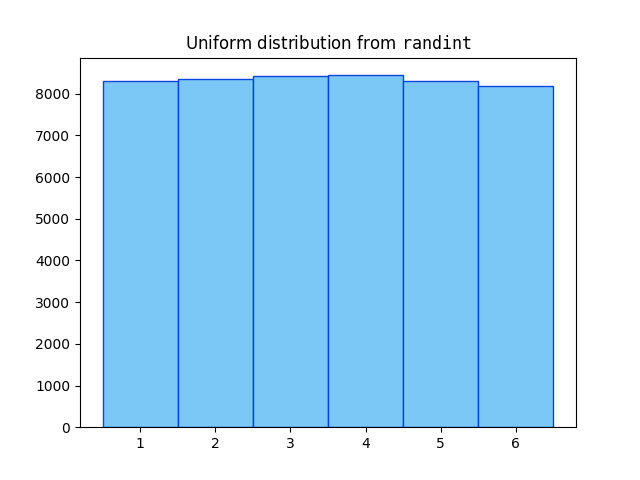
\includegraphics[width=0.7\textwidth]{figures/uniform}
\caption{Uniform distribution generated with \texttt{random.randint} function.}
\label{fig:uniform_dist}
\end{figure}
    
Another module that will be used to generate random numbers is \texttt{numpy}. It has similar functionalities to \texttt{random} but in some cases it fits better to our needs.    
Below an example with \texttt{numpy.random.normal} which throws random numbers sampled from a normal distribution ($\mathcal{N}(0, 1)$), the result is shown in Fig.~\ref{fig:gauss_dist}.

\begin{ipython}
from numpy.random import normal
from matplotlib import pyplot as plt

gauss = normal(size=50000)

plt.hist(gauss, 100, range=[-4, 4])
plt.title("Example of Gaussian distribution from numpy")
plt.show()
\end{ipython}

\begin{figure}
\centering
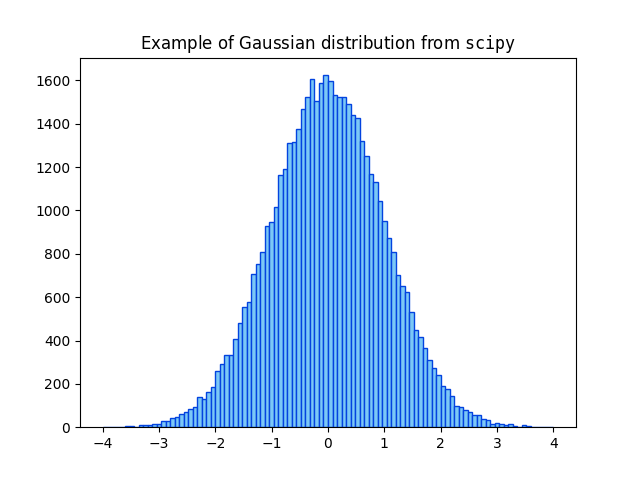
\includegraphics[width=0.7\textwidth]{figures/standard_normal}
\caption{Normal distribution generated with \texttt{numpy.random.normal} function.}
\label{fig:gauss_dist}
\end{figure}

%\hypertarget{acceptance-rejection-method}{%
%\subsubsection{Acceptance-Rejection
%	Method}\label{acceptance-rejection-method}}
%
%The acceptance-rejection method was proposed by von Neumann in 1951 and
%is used in order to generate random variables that follow a probability
%density function denoted by \(f(x)\).
%
%Given a target distribution \(f(x)\), the acceptance-rejection
%method generates samples according to \(f(x)\) by first of all
%generating samples from a more suitable distribution \(g(y)\).
%Afterwards a random subset of these generated samples is rejected
%according to certain rejection rules. Thereby the choice of this
%rejection rule, or let us call it rejection approach, will be decisive
%if the accepted samples will eventually be distributed according to
%\(f(x)\). The property \(f(x) \leq c\cdot g(x)\), for some constant
%\(c\), tells us now how to generate samples from \(g(y)\). Therefore, we
%conclude that in the acceptance-rejection method a sample \(Y\) is
%generated from \(g\) and at the same time accepted with probability
%\(f(Y)/cg(Y)\). The generic implementation, i.e.~the algorithm of the
%acceptance-rejection method that we can use to sample from density \(f\)
%using candidates from \(g\), can be stated as follows:
%
%\begin{enumerate}
%\def\labelenumi{\arabic{enumi}.}
%\tightlist
%\item
%generate the sample \(Y\) from the distribution with density \(g\)
%\item
%generate \(u\) from \(U[0,1]\), which must be independent of \(Y\)
%\item
%if \(u\leq f(Y)/cg(Y)\), then deliver \(X = Y\), otherwise return to
%step 1.
%\end{enumerate}

\section{Monte Carlo Simulation Examples}
\label{example-of-monte-carlo-simulation}

In this Section we go through some applications of the Monte Carlo method.

\subsection{Probability to Draw Two Kings From a Deck}
According to the frequentist approach, we can calculate the probability of an event as the ratio of the number of favorable outcomes (number of successes) and the number of all possible outcomes. 

Imagine we would like to determine the probability of drawing consecutively two kings from a deck of cards. At the beginning there are 40 cards (i.e. the entire deck) with 4 possible kings, so the probability to get the first king is $4/40=10\%$. Next, assuming we've got a king the first time, we are left with 39 cards and 3 kings only, so the probability to get the second king is $3/39=7.7\%$. Since we want both events to happen, the final probability is the product of the two:

\begin{equation*}
P_\textrm{two kings} = \frac{4}{40} \cdot \frac{3}{39} = \frac{1}{130} \approx 0.77\%
\end{equation*}

Let's now try to estimate the same probability with a MC simulation, following the steps outlined above.

In this case the domain is a deck of cards. To create a virtual deck we define a list of card for a single suit and then "multiply" the list by four. The seed is set to 1 to make the exercise reproducible.
We draw randomly cards with uniform probability since the deck is fair (all cards have the same probability to be drawn). 
We plan to do one million simulations; each time, with the \texttt{sample} function, we pick up two cards from the virtual deck (for debugging purpose the first ten trials are printed on screen). Check if the card pair is \texttt{['K', 'K']} and in case increase the counter of successes. Finally just print \texttt{successes/trials} which is the sought probability.

\begin{ipython}
from random import sample, choices, seed

seed(1)
deck = ["A", "2", "3", "4", "5", "6", "7", "J", "Q", "K"] * 4

trials = 1000000
successes = 0

for i in range(trials):
    cards = sample(deck, k=2)
    if i < 10:
        print (cards)
    if cards == ["K", "K"]:
        successes += 1

print ("The probability to draw two kings is {:.4f}".format(successes/trials))
\end{ipython}
\begin{ioutput}
['Q', '7']
['5', '7']
['J', '2']
['Q', 'A']
['5', '4']
['7', '2']
['2', '5']
['J', 'Q']
['A', 'Q']
['J', '5']

The probability to draw two kings is 0.0077
\end{ioutput}

The result is in agreement with the theoretical expectations. Further considerations about this result in Section~\ref{sec:confidence_interval}.

\subsection{Determine $\pi$}
\label{determine-pi}

Also in this example we know what the result has to be: $\pi\approx 3.141592653589793\ldots$ In order to get an estimate through MC simulation of this famous constant a geometric approach can be considered (by the way this very same technique can be used to measure any arbitrary shape). Imagine a circle of radius $r$ which is inscribed in a square with side length $2r$, see Fig.~\ref{fig:circle_inscribed}.

\begin{figure}[htb]
\centering
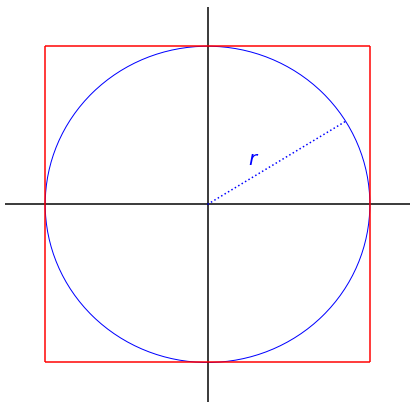
\includegraphics[width=0.5\textwidth]{figures/circle_inscribed}
\caption{A circle of radius $r$ inscribed in a square of side length $2r$.}
\label{fig:circle_inscribed}
\end{figure}

Computing the ratio of the two figure areas

\begin{equation}
\frac{\textrm{Area Circle}}{\textrm{Area Square}} = \frac{\pi r^2}{4r^2} = \frac{\pi}{4} 
\end{equation}

The algorithm to approximate $\pi$ should then be

\begin{itemize}
\item select 2 random numbers, $x_1$ and $x_2$, from the interval
$[-r,r]$; 
\item determine if the point defined by the ordered pair $(x_1, x_2)$ lies within or on the circle, keeping track both of the total number of tested points and of those satisfying the condition $\sqrt{x_1^2 + x_2^2}\leq r$; 
\item approximate the ratio of the areas by the number of points within or on the circle divided by the total number of tested points; 
\item multiply the approximated area by 4 to get $\pi$.
\end{itemize}

\begin{ipython}
from random import random, seed
from math import sqrt

seed(2)
def simulation(trials):
  r = 1
  in_circle = 0.0
  for _ in range(trials):
      x1 = -r + random()*2*r
      x2 = -r + random()*2*r
      distance = sqrt(x1**2 + x2**2)
      if distance <= r:
          in_circle += 1
  return in_circle 

trials = 10000
in_circle = simulation(trials)
print ("Approx. pi: {}".format(in_circle/trials*4))  
\end{ipython}
\begin{ioutput}
Approx. pi: 3.1524
\end{ioutput}

A general consideration that we can make is that the lower is the probability we try to estimate with MC the higher has to be the number of simulations. 
The result precision indeed depends on the amount of "successes" and if the success probability is small, many trials are needed. 

This can be simply checked by playing with the number of simulations in the previous examples. We may run an entire set without getting two consecutive kings, nevertheless we cannot conclude there is zero probability of such event.

The only conclusion we can draw is that, despite its undoubted power, Monte Carlo simulation is not always the best approach to follow, especially for computationally heavy experiments. Many times indeed the simulation of a single experiment requires a lot of computing resources (and time) and it may not be practical to embark into such a large simulation.

In the following example it is apparent how increasing the number of simulations in a single experiment the approximation precision improves. In Fig.~\ref{fig:circle_approx} it is shown graphically the results with 100, 1000, 10000, 100000 and 1000000 simulations.

\begin{ipython}
from random import random, seed
from math import sqrt
import numpy as np, time

seed(1)
trials=[100, 1000, 10000, 100000, 1000000]
for i, t in enumerate(trials):
    t1 = time.time()
    in_circle = simulation(t)
    t2 = time.time() - t1
    print ("pi={:.6f} {:.4f}s".format(in_circle/t*4, t2))
\end{ipython}
\begin{ioutput}
pi=3.120000 0.0001s
pi=3.096000 0.0012s
pi=3.121200 0.0147s
pi=3.139560 0.1997s
pi=3.142136 1.0671s
\end{ioutput}

\begin{figure}[htb]
\centering
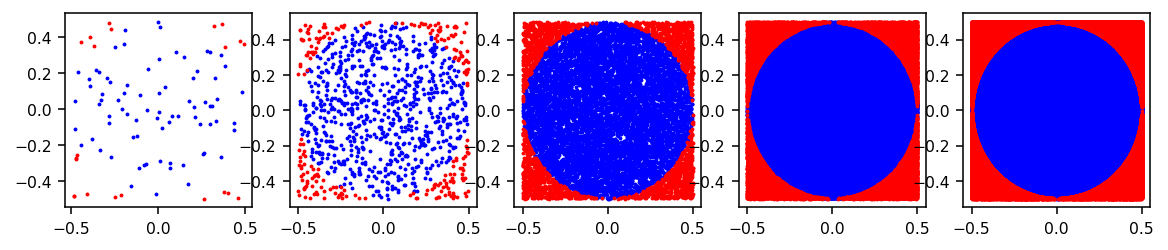
\includegraphics[width=1\textwidth]{figures/mc_vs_n_experiments}
\caption{Graphical representation of geometrical approximation of $\pi$. Results are reported for $N = 100, 1000, 10000, 100000, 1000000$ simulations. It is clear how the result improves with $N$.}
\label{fig:circle_approx}
\end{figure}

In this case the simulation is so simple that even in the larger case ($N=1000000$) the program runs for about a second only.

\section{Accuracy of Monte Carlo Simulation}
\label{sec:confidence_interval}

Let's go back to the card example and imagine that you didn't know how much is the probability of getting two consecutive K from a deck of 40 cards. 
    
\begin{ipython}
from random import sample, seed

seed(97)
def deck_sim(trials):
    successes = 0.0
    for _ in range(trials):
        cards = sample(deck, 2)
        if cards == ['K', 'K']:
            successes += 1
    return successes

trials = 10000
successes = deck_sim(trials)
print (successes/trials)
\end{ipython}
\begin{ioutput}
0.0084
\end{ioutput}

What can be concluded from the result of a single MC experiment ?
Unfortunately not much, but a famous theorem come to rescue us.
The central limit theorem~\cite{bib:central_limit} states that if we have $Y_1, Y_2,\dots, Y_n$ which are $n$ random samples from a distribution $Y$ with true mean $\mu$ and variance $\sigma^{2}$, then with $n$ sufficiently large,

\begin{equation*} 
\mu_n = \cfrac{1}{n}\sum_i^n Y_i
\end{equation*}
has approximately a normal distribution $\mathcal{N}(\mu, \sigma^2/n)$.

This means that if one repeats the same MC experiment many times (changing the random number generator seed otherwise we are always repeating the \emph{same} experiment) would obtain results normally distributed around the \emph{true} value $\mu$.
We can check the central limit theorem by repeating many times the MC experiment with our virtual deck and see how the distribution of $\mu_n$ behaves.

\begin{ipython}
import numpy as np
from random import sample, seed

experiments = 1000
trials = 10000
r = []

for e in range(experiments):
	seed(e)
    successes = deck_sim(trials)
    r.append(successes/trials)

print ("Mean: {:.6f}".format(np.mean(r)))
print ("Std : {:.6f}".format(np.std(r)))
\end{ipython}
\begin{ioutput}
Mean:  0.007688
Std :  0.000871
\end{ioutput}

Looking at Fig.~\ref{fig:repeated_MC} it is clear that the various results are distributed as a Gaussian (in this example the distribution is still a bit asymmetric but it will eventually become Gaussian running more simulations).

\begin{figure}[htb]
\centering
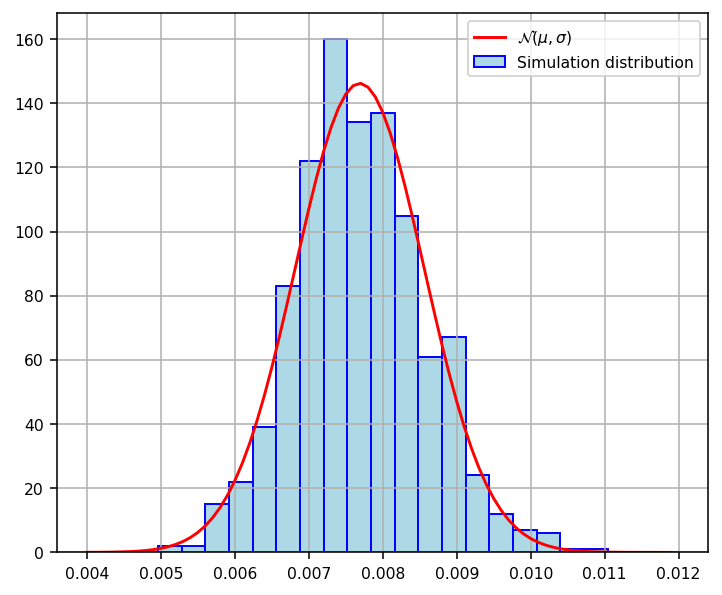
\includegraphics[width=0.7\textwidth]{figures/experiment_distribution}
\caption{Distribution of the results of 1000 experiments.}
\label{fig:repeated_MC}
\end{figure}

From the central limit theorem hence: 

\begin{equation}
\mu_n - \mu \approx \mathcal{N}(0, \sigma^2/n)
\end{equation}

From the previous equation and remembering the definition of quantiles~\ref{sec:quantile-function} it is possible to define an interval such that there is a certain probability to find $\mu$ in there. Referring to Fig.~\ref{fig:confidence_interval} we can write:

\begin{equation}
P\left(\mu_n - 1.96\frac{\sigma}{\sqrt{n}}\le \mu \le \mu_n + 1.96\frac{\sigma}{\sqrt{n}}\right) = 0.95
\end{equation}
(which corresponds to the pink area).

\begin{figure}[htb]
\centering
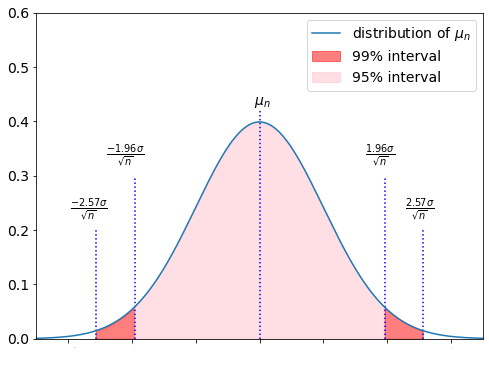
\includegraphics[width=0.7\textwidth]{figures/confidence_interval}
\caption{Confidence interval for a MC experiment.}
\label{fig:confidence_interval}
\end{figure}

This interval is called \textbf{95\% confidence interval} because it covers 95\% of the total area under the Gaussian. It can be interpreted like the following: if you repeat many times a simulation, the fraction of calculated confidence intervals that contains the true parameter $\mu$ would tend toward 95\%.

The most commonly used intervals are 99\% and 95\% confidence level and are respectively defined as \(\pm \cfrac{2.57\sigma}{\sqrt{n}}\) and \(\pm \cfrac{1.96\sigma}{\sqrt{n}}\).

To construct an interval with a custom confidence level $\alpha$, we have to find a number $A$ such that
\begin{equation}
\Phi(A) = 1 - \frac{1-\alpha}{2}\quad\implies\quad A = \Phi^{-1}\left(\cfrac{1+\alpha}{2}\right)
\label{for:A}
\end{equation}
then the $\alpha$-confidence interval guarantees
\begin{equation}
P(\mu - A\sigma \le X \le \mu+ A\sigma) = \alpha 
\end{equation}

Below an example of how to compute a confidence level in \texttt{python} given a set of simulation results (the inverse of the Gaussian CDF $\Phi^{-1}$, used in Eq.~\ref{for:A}, is computed with the method \texttt{norm.ppf()}, see Section~\ref{sec:quantile-function}).

\begin{ipython}
import numpy as np
from scipy.stats import norm

samples = [1.,2.,3.,4.,4.,4.,5.,5.,5.,5.,4.,4.,4.,6.,7.,8.]
alpha = 0.95
X = np.array(samples)
A = norm.ppf((1 + alpha)/2)
m, se = np.mean(X), np.std(X)
h = A*se/np.sqrt(len(samples))
print ("{:.0f}% confidence int.: {:.3f} +- {:.3f}".format(alpha*100, m, h))
\end{ipython}
\begin{ioutput}
95% confidence int.: 4.437 +- 0.812
\end{ioutput}

The confidence interval is used to assess the accuracy of a Monte Carlo simulation. From what has been said above the uncertainty on our best estimate of $\mu$ is $\sqrt{\cfrac{\sigma^2}{n}}=\cfrac{\sigma}{\sqrt{n}}$ where \(\sigma^2 = \mathrm{Var}(Y)\).

While it is obvious that the estimate should get worse with increased variance and better with bigger sample size, this equation gives us the exact scaling. Indeed the uncertainty formula tells us that to get one more decimal digit of accuracy (i.e. an error one tenth as large) requires a 100-fold increase in computation. To get three more digits of accuracy requires one million times as much computation. From that it is clear that Monte Carlo is poorly suited for problems that must be answered with high precision.

\section{Integration by Monte Carlo}
\label{sec:integration}
Function integration in \texttt{python} can be performed using \texttt{scipy.integrate.quad}. 
This method takes in input: the function to integrate, the integration limits and, if needed, optional arguments for the integrand (see Section~\ref{sec:kwargs_args}). Since it is a numerical integration the result will be a tuple with the actual result and its associated error.

For example imagine to integrate
\begin{equation*}
f(x) = \int_{0}^{\infty}\frac{e^{-x}}{\left(a + (x-1)^2\right)}~dx
\end{equation*}
for $a=3$.

\begin{ipython}
import numpy as np
from scipy.integrate import quad
	
def f(x, a):
    return np.exp(-x)/(a+(x-1)**2)
	
s = quad(f, 0, np.inf, args=(3,))
print (s)
\end{ipython}
\begin{ioutput}
(0.2802620835548487, 1.5887625490132047e-09)
\end{ioutput}

Sometimes it may be useful to calculate the approximate result of an integral of a function $f$ through Monte Carlo simulation. The technique relies on the fact that the average of $f$ calculated in the integration interval can be expressed as

\begin{equation}
<f(x)> = \frac{1}{b-a} \int_{a}^{b} f(x) \,dx
\end{equation}
Rearranging the terms
\begin{equation}
\int_{a}^{b} f(x) \,dx = 
(b-a) <f(x)> \approx (b-a) \frac{1}{N} \sum_{i=1}^{N} f(x_i)
\end{equation}
Then the integral can be computed by sampling values of $x$ from a uniform distribution between $[a,b]$, average the evaluations of $f(x)$ and then multiplying the result by $(b-a)$.

Considering the previous integral

\begin{ipython}
import random 
import numpy as np

def myrand(llim, ulim, n):
    return np.random.uniform(size=n)*(ulim-llim) + llim

def f(x, a):
    return np.exp(-x)/(a+(x-1)**2)

def integration_mc(f, args, llim, ulim, iter=10000):
    vals = f(myrand(llim, ulim, iter), *args)
    return (ulim-llim)*np.mean(vals)

print (integration_mc(f, (3,), 0, 5, 1000000))
\end{ipython}
\begin{ioutput}
0.28061306413101306
\end{ioutput} 
 
Although there are various improvements that can be added to our simple MC implementation, the result that we obtained is in good agreement with the one from the \texttt{python} implementation.  
 
\section*{Exercises}
\begin{question}
Using the function \texttt{randint} of the module \texttt{random} make a Monte Carlo simulation of rolling three dices to check the probability of getting the same values on the three of them.
From the probability theory you should expect:

\[P_{d1=d2=d3} = \frac{1}{6}\cdot\frac{1}{6}\cdot\frac{1}{6}\cdot 6 = \frac{1}{36} = 0.0278\]
\end{question}

\cprotEnv\begin{solution}
\begin{ipython}
from random import seed, randint

seed(1)
trials = 10000000
success = 0

for _ in range(trials):
    d1, d2, d3 = randint(1, 6), randint(1, 6), randint(1, 6)
    if d1 == d2 and d2 == d3:
        success += 1

print ("The probability to get three equal dice is {:.4f}".format(success/trials))

The probability to get three equal dice is 0.0278
\end{ipython}
\end{solution}

\begin{question}
Two fair dice are rolled, find the probability that their sum is:
\begin{enumerate}[start=1]
	\item equal to 1;
	\item equal to 4;
	\item less than 13.
\end{enumerate}
	
\noindent\textbf{Hint:} the possible combinations of the outcomes of two dice are 36 (to realize it you can simply think that for each one of the six faces of the first die you have six possible faces of the second hence $6\cdot 6=36$). It is not possible to get 1 since the dice have no face with 0 so the first probability should come out 0. The sum of the two dice is always less than 13 (the maximum is 12\ldots) so the answer to point 3 is 1. We can get a sum of 4 in 3 cases (1-3, 3-1 or 2-2) so the expected probability is $3/36=1/12=0.0833$
\end{question}

\cprotEnv\begin{solution}
\begin{ipython}
import random

random.seed(1)
successes = {"=1":0.0, "=4":0.0, "<13":0.0}
trials = 100000

for _ in range(trials):
    d1 = random.randint(1, 6)
    d2 = random.randint(1, 6)

    if (d1 + d2) == 1:
        successes["=0"] += 1.0
    if (d1 + d2) == 4:
        successes["=4"] += 1.0
    if (d1 + d2) < 13:
        successes["<13"] += 1.0

for k,v in successes.items():
    print ("P({}): {:.3f}".format(k, v/trials))

P(=1): 0.000
P(=4): 0.084
P(<13): 1.000
\end{ipython}
\end{solution}

\begin{question}
There are 60 chemical flasks in the laboratory, 6 of which are incorrectly labeled. What is the chance that if we randomly choose 5 flasks, exactly 3 of them will be labeled correctly ?

\noindent\textbf{Hint:} the probability is approximately 0.5 \%.
\end{question}

\cprotEnv\begin{solution}
\begin{ipython}
import random

flasks = ["C"]*54 + ["U"] * 6
random.seed(1)
trials = 1000
success = 0.

for _ in range(trials):
    draw = random.sample(flasks, 5)
    if draw.count("U") == 3:
        success += 1.

print ("Probability: {:.3f}%".format(success/float(trials)*100))

Probability: 0.499%
\end{ipython}
\end{solution}

\begin{question}
Given the following historical series (1895-2020) find average September temperature in US and report the 99\% confidence interval of your measure.
\noindent
Input (temperatures are in Fahrenheit degrees): \href{https://raw.githubusercontent.com/matteosan1/finance_course/develop/libro/input_files/histo_temp.csv}{histo\_temp.csv}
\end{question}

\cprotEnv\begin{solution}
\begin{ipython}
from scipy.stats import norm
import numpy as np
import pandas as pd

# first download the input file
df = pd.read.csv("histo_temp.csv")
temperatures = df['T'].to_array()
alpha = 0.99

A = norm.ppf((1 + alpha)/2)
m, se = np.mean(temperatures), np.std(temperatures)
h = A*se/np.sqrt(len(temperatures))

print ("Avg temperature in September (US): {:.1f}".format(m))
print ("{:.1f}% confidence interval: +- {}".format(alpha*100, h))
Avg temperature in September (US): 65.1
99% confidence interval: +- 0.3
\end{ipython}
\end{solution}

\begin{question}
Using the function \texttt{normal} of \texttt{numpy.random} simulate the price of a stock which evolves according to a log-normal stochastic process with a daily rate of return \(\mu=0.1\) and a volatility \(\sigma=0.15\) for 30 days.
Also plot the price. Try to play with \(\mu\) and \(\sigma\) to see how the plot changes.
\end{question}

\cprotEnv\begin{solution}
\begin{ipython}
from numpy.random import normal, seed
from matplotlib import pyplot as plt
import math

S = 100
mu = 0.1
sigma = 0.15
T = 1
seed(1)

historical_series = [S]
for i in range(30):
    S = S * math.exp((mu - 0.5 * sigma * sigma) * T +
        sigma * math.sqrt(T) * normal())
    historical_series.append(S)

plt.plot(range(31), historical_series)
plt.xlabel("days")
plt.ylabel("Price of stock X")
plt.show()
\end{ipython}

\begin{figure}[htbp]
\begin{center}
  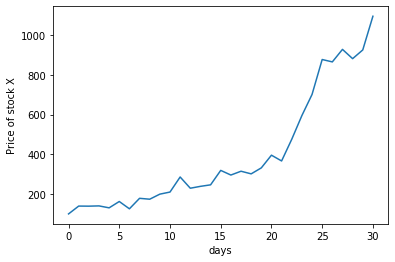
\includegraphics[width=0.7\linewidth]{figures/lesson6_solutions_5_0.png}
\end{center}
\end{figure}
\end{solution}


\begin{thebibliography}{9}
\bibitem{bib:monte_carlo}\href{https://www.youtube.com/watch?v=OgO1gpXSUzU}{\emph{Monte Carlo Simulation}}, MIT Course [Online]
\bibitem{bib:central_limit} \href{https://en.wikipedia.org/wiki/Central_limit_theorem}{\emph{Central Limit Theorem}}, Wikipedia [Online]
\bibitem{bib:confidence_interval}\href{https://www.statisticshowto.com/probability-and-statistics/confidence-interval}{\emph{Confidence Interval: How to Find a Confidence Interval: The Easy Way!}}, Statistic Howto [Online]
\end{thebibliography}









